\documentclass[11pt,a4paper,fleqn]{article}
\usepackage[utf8]{inputenc}
\usepackage{bsymb}
%usepackage[space]{ctex}
\usepackage{natbib}
\usepackage{graphicx}
\usepackage{algorithmic_pf}
\usepackage{indentfirst}
\usepackage[export]{adjustbox}
\usepackage{etoolbox}
\expandafter\patchcmd\csname Gin@ii\endcsname
  {\setkeys {Gin}{#1}}
  {%
    \setkeys {Gin}
      {max width=\textwidth,max height=.5\textwidth,keepaspectratio,#1}%
  }
  {}{}
\title{Homework 6}

\author{10175101126,10175101226,10175101117}
\date{April 2019}
\setkeys{Gin}{max width=\linewidth}
\begin{document}
\maketitle

\section{ Exercise 1}
\noindent
$[x:\in S;$ if $P(x)$ then $y:=a$ else $y:=b$ end]$Q(x,y)$\\
$x^{'}\in S\vdash $[if $P(x^{'})$ then $y:=a$ else $y:=b$ end]$Q(x^{'},y)$\\
$x^{'}\in S,P(x^{'})\vdash [y:=a]Q(x^{'},y)$\\
$x^{'}\in S,P(x^{'})\vdash Q(x^{'},a)$\\
$x^{'}\in S,\neg P(x^{'})\vdash [y:=b]Q(x^{'},y)$\\
$x^{'}\in S,\neg P(x^{'})\vdash Q(x^{'},b)$
\section{Exercise 2}
\subsection{Prove the feasibility rules}
\noindent
$PRE,f(r)\not=v,f(r)<v,r\in p\upto q,v\in f[p\upto q]\vdash r+1\upto q \not=\emptyset$\\
To prove it, we need to prove $r\not=q$ first.\\
$PRE,f(r)\not=v,f(r)<v,r\in p\upto q,v\in f[p\upto q]\vdash r\not=q$\\
$PRE,f(r)<v,r=q,r\in p\upto q,v\in f[p\upto q]\vdash f(r)=v\quad\text{CT2}$\\
$PRE,f(q)<v,q\in p\upto q,v\in f[p\upto q]\vdash f(r)=v\quad\text{EQL}$\\
since f is increasing,$f(q)<v$ means $v\not\in f[p\upto q].$\\  
$PRE,v\not\in f[p\upto q],q\in p\upto q,v\in f[p\upto q]\vdash f(r)=v\quad\text{CT1}$\\
$PRE,f(r)\not=v,f(r)<v,r\in p\upto q,v\in f[p\upto q],r\not=q\vdash r+1\upto q \not=\emptyset\quad\text{AH}$\\
Obvious,since $r<q$.\\
$PRE,f(r)\not=v,f(r)>v,r\in p\upto q,v\in f[p\upto q]\vdash p\upto r-1 \not=\emptyset$\\
To prove it, we need to prove $r\not=p$ first.\\
$PRE,f(r)\not=v,f(r)> v,r\in p\upto q,v\in f[p\upto q]\vdash r\not=p$\\
$PRE,f(r)> v,r=p,r\in p\upto q,v\in f[p\upto q]\vdash f(r)=v\quad\text{CT2}$\\
$PRE,f(p)> v,p\in p\upto q,v\in f[p\upto q]\vdash f(p)=v\quad\text{EQL}$\\
since f is increasing,$f(p)>v$ means $v\not\in f[p\upto q].$\\  
$PRE,v\not\in p\upto q,p\in p\upto q,v\in f[p\upto q]\vdash f(p)=v\quad\text{CT1}$\\
$PRE,f(r)\not=v,f(r)>v,r\in p\upto q,v\in f[p\upto q],r\not=p\vdash p\upto r-1 \not=\emptyset$\\
Obvious,since $r>p$.\\
\subsection{Propose a variant and prove}
\noindent              
we propose the q-p as the variant.\\
\text{NAT:}\\
$\ldots,v\in ran(f),v\in f[p\upto q]\vdash q-p\in\mathbb{N}$\\
Obvious,since $p\upto q\not=\emptyset$,$p\leq q$.\\
\text{VAR}:\\
$PRE,f(r)\not=v,f(r)<v,r\in p\upto q,v\in f[p\upto   q]\vdash [p:=r+1]q-p<q-p$\\
$PRE,f(r)\not=v,f(r)<v,r\in p\upto q,v\in f[p\upto   q]\vdash q-(r+1)<q-p$\\
$PRE,f(r)\not=v,f(r)<v,r\in p\upto q,v\in f[p\upto   q]\vdash (r+1)>p$\\
Obvious, since $r\in p\upto q,r\geq p$.\\
$PRE,f(r)\not=v,f(r)\geq v,r\in p\upto q,v\in f[p\upto   q]\vdash [q:=r-1]q-p<q-p$\\
$PRE,f(r)\not=v,f(r)\geq v,r\in p\upto q,v\in f[p\upto   q]\vdash r-1-p<q-p$\\
$PRE,f(r)\not=v,f(r)\geq v,r\in p\upto q,v\in f[p\upto   q]\vdash r-1<q$\\
Obvious, since $r\in p\upto q,r\leq q$.
\section{Exercise 3}
\subsection{ Prove that the three assignments to r are indeed }
\noindent
we know that the three sets are not empty set because of the feasibility rule.\\
$\ldots\vdash [r:=(n-1+0)/2]r\in 0\upto n-1$\\
$\ldots\vdash (n-1+0)/2\in 0\upto n-1$\\
Obvious, since $n>0$\\
$\ldots,r+1\upto q\not=\emptyset\vdash [r:=(r+1+q)/2]r\in r+1\upto q$\\
$\ldots,r+1\upto q\not=\emptyset\vdash (r+1+q)/2\in r+1\upto q$\\
$\ldots,(r+1+q)/2\not\in r+1\upto q\vdash r+1\upto q=\emptyset\quad\text{CT2}$\\
$\ldots,(r+1+q)/2> q \lor (r+1+q)/2< r+1\vdash r+1\upto q=\emptyset$\\
$\ldots,(r+1+q)/2> q \vdash r+1\upto q=\emptyset\quad\text{OR\_H}$\\
$\ldots,r+1>q \vdash r+1\upto q=\emptyset$\\
Obvious that is true\\
$\ldots,(r+1+q)/2< r+1 \vdash r+1\upto q=\emptyset\quad\text{OR\_H}$\\
$\ldots,q<r+1 \vdash r+1\upto q=\emptyset$\\
Obvious that is true\\
$\ldots,p\upto r-1\not=\emptyset\vdash [r:=(p+r-1)/2]r\in p\upto r-1$\\
$\ldots,p\upto r-1\not=\emptyset\vdash (p+r-1)/2\in p\upto r-1$\\
$\ldots,(p+r-1)/2\not\in p\upto r-1\vdash p\upto r-1=\emptyset\quad\text{CT2}$\\
$\ldots,(p+r-1)/2> r-1 \lor (p+r-1)/2< p\vdash p\upto r-1=\emptyset$\\
$\ldots,(p+r-1)/2> r-1 \vdash p\upto r-1=\emptyset\quad\text{OR\_H}$\\
$\ldots,p>r-1 \vdash p\upto r-1=\emptyset$\\
Obvious that is true\\
$\ldots,(p+r-1)/2< p \vdash p\upto r-1=\emptyset\quad\text{OR\_H}$\\
$\ldots,r-1<p \vdash p\upto r-1=\emptyset$\\
Obvious that is true\\
\subsection{Translate the final program to C and execute it}
\noindent
Program is listed here:
\begin{figure}[h!]
\centering
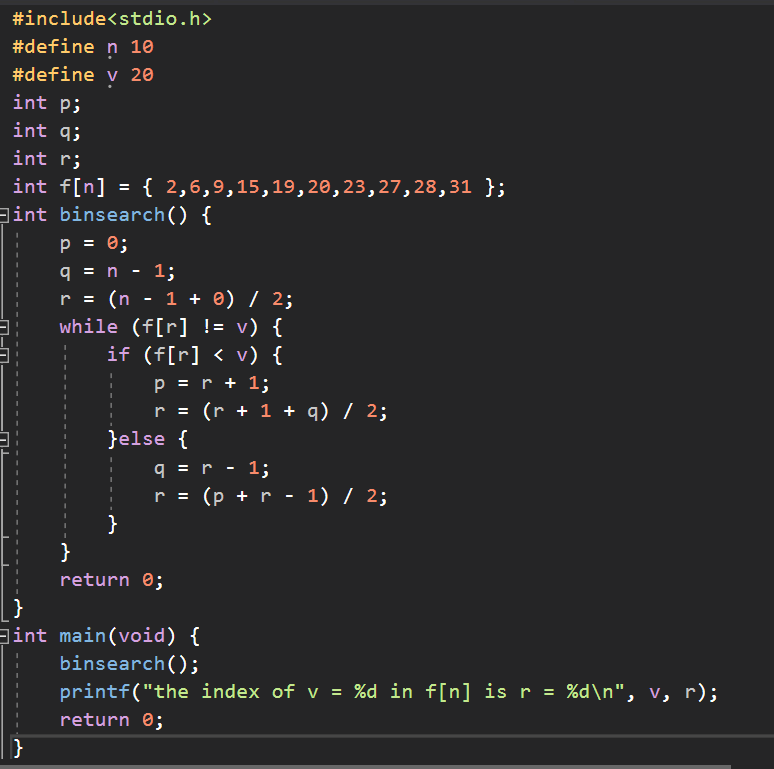
\includegraphics{1.png}
\caption{ write in c}
\label{fig}
\end{figure}
\begin{figure}[h!]
\centering
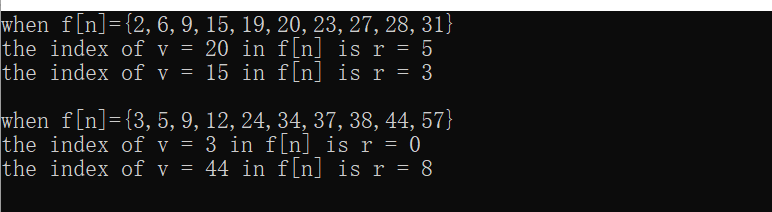
\includegraphics{2.png}
\caption{ excute with some f and v}
\label{fig}
\end{figure}


%\bibliographystyle{plain}
%\bibliography{references}
\end{document}
